\scanpage{68}\mspage{67}
\deleted{On a une notion de \unsure{``c|``C|``6}}

Toute partie de $\mathcal F$ (resp $M$) est contenue dans une partie saturée \unsure{minimale} (parmi \unsure{celles|telles} la contenant), qui \deleted{s'appelle \unsure{du|de}} n'est autre que le cosupport du cosupport, et s'appelle aussi son support. Les parties saturées sont celles qui sont égales au support, ou au cosupport, d'une partie. L'application . $\operatorname{cosup}$ définit une \unsure{bij\inserted{e}ction} de l'ens des parties \unsure{saturées|saturée} \unsure{sur} elles $=$, renversant la relation d'inclusion.

On désigne par $\Sigma$ l'ens des \uline{supports} \uline{virtuels}, ou parties saturées
% Figure R3-M0-insertion: the curved oblique insertion arm has no arrowhead.
\figure{%
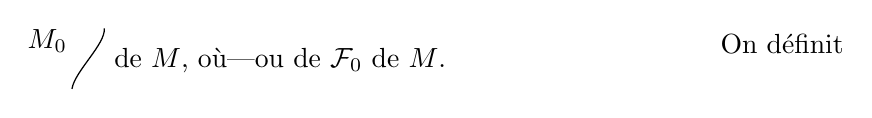
\begin{tikzpicture}[x=1cm,y=1cm]
\node[anchor=base west,inner sep=0pt] at (0,0.24) {\inserted{$M_0$}};
\node[anchor=base west,inner sep=0pt] at (1.1,0) {de $M$, \unsure{où|ou} \deleted{\unsure{de}} $\mathcal F_0$ de $M$.};
\node[anchor=base west,inner sep=0pt] at (8.8,0.18) {\deleted{On \unsure{définit}}};
\draw[line width=0.45pt] (0.98,0.50) .. controls (1.00,0.30) and (0.60,-0.05) .. (0.57,-0.27);
\end{tikzpicture}%
}
\deleted{L'application de cosupport \unsure{de|d}} On \unsure{désidentifie} $\Sigma$ de \deleted{$\unsure{\mathcal F}$} ses deux \unsure{réalisations} (comme \unsure{partie|parties} de $\unsure{\mathscr P|\mathcal P|\wp}(M)$, ou de $\mathscr P(\mathcal F)$) et on écrit, pour $\sigma\in\Sigma$
\[
M_\sigma\subset M,\qquad\mathcal F_\sigma\subset\mathcal F
\]

Dans $\Sigma$, \deleted{pour} la notion de cosupport est une
% Figure R3-worked-anti: one worked suffix, with a drawn overstrike; an older complete word cannot be isolated.
\figure{%
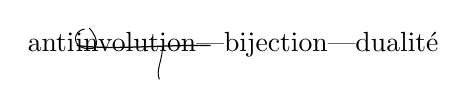
\begin{tikzpicture}[x=1cm,y=1cm]
\node[anchor=base east,inner sep=0pt] at (0,0) {anti};
\node[anchor=base west,inner sep=0pt] at (0,0) {\unsure{involution|bijection|dualité}};
\draw[line width=0.45pt] (0.02,0.08) .. controls (0.48,0.02) and (1.10,0.09) .. (1.72,0.08);
\draw[line width=0.35pt] (0.12,0.29) .. controls (-0.03,0.27) and (-0.06,0.04) .. (0.18,0.04) .. controls (0.34,0.03) and (0.26,0.22) .. (0.18,0.30);
\draw[line width=0.35pt] (1.11,0.07) .. controls (1.11,-0.11) and (1.02,-0.24) .. (1.07,-0.35);
\end{tikzpicture}%
}
d'ens. ordonnés. Dans $\Sigma$, on a des $\mathrm{Inf}$ quelconques (c'est l'intersection des parties de $M$, ou de $\mathcal F$), et des $\mathrm{Sup}$ quelconques (c'est la partie saturée
